% Created 2022-06-06 Mon 07:40
% Intended LaTeX compiler: pdflatex
\documentclass[presentation,aspectratio=169, usenames, dvipsnames]{beamer}
\usepackage[utf8]{inputenc}
\usepackage[T1]{fontenc}
\usepackage{graphicx}
\usepackage{grffile}
\usepackage{longtable}
\usepackage{wrapfig}
\usepackage{rotating}
\usepackage[normalem]{ulem}
\usepackage{amsmath}
\usepackage{textcomp}
\usepackage{amssymb}
\usepackage{capt-of}
\usepackage{hyperref}
\usepackage{khpreamble}
\usepackage{amssymb}
\usepgfplotslibrary{groupplots}
\newcommand*{\shift}{\operatorname{q}}
\definecolor{ppc}{rgb}{0.1,0.1,0.6}
\definecolor{iic}{rgb}{0.6,0.1,0.1}
\definecolor{ddc}{rgb}{0.1,0.6,0.1}
\usetheme{default}
\author{Kjartan Halvorsen}
\date{\today}
\title{Block-diagram algebra}
\hypersetup{
 pdfauthor={Kjartan Halvorsen},
 pdftitle={Block-diagram algebra},
 pdfkeywords={},
 pdfsubject={},
 pdfcreator={Emacs 26.3 (Org mode 9.4.6)}, 
 pdflang={English}}
\begin{document}

\maketitle


\section{Block stuff}
\label{sec:org06f72d5}

\begin{frame}[label={sec:org0f0cb78}]{The model of the Hummer EV}
\begin{columns}
\begin{column}{0.5\columnwidth}
\begin{block}{ODE}
\[m\dot{y} = -2kv_0y + u,\]
\[ \dot{y} + \frac{2\cdot 1.44\cdot 22}{5000} y = \frac{1}{5000} u, \]
\[ \dot{y} + 0.013 y = 0.0002u, \]
\[ 78.9\dot{y} + y = 0.016u. \]
\end{block}

\begin{block}{Laplace transform}
\[ (78.9s + 1) Y(s) = 0.016 U(s) \]
\end{block}
\end{column}

\begin{column}{0.5\columnwidth}
\begin{block}{Transfer function}
\[  Y(s) = \underbrace{\frac{\overbrace{0.016}^K}{ \underbrace{78.9}_\tau s + 1}}_{G(s)} U(s) \]
\end{block}

\begin{block}{Block diagram}
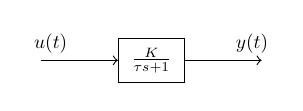
\begin{tikzpicture}[scale=0.7, transform shape, block/.style={draw, minimum width=12mm, minimum height=8mm},]
  \node[block] (plant) {$\frac{K}{\tau s + 1}$};
  \draw[->] (plant) ++ (-2cm, 0) -- node[very near start, above] {$u(t)$} (plant);
  \draw[->] (plant) -- node[very near end, above] {$y(t)$} ++(2cm, 0);
\end{tikzpicture}
\end{block}
\end{column}
\end{columns}
\end{frame}


\begin{frame}[label={sec:org72eb2af}]{Feedback control}
\begin{center}
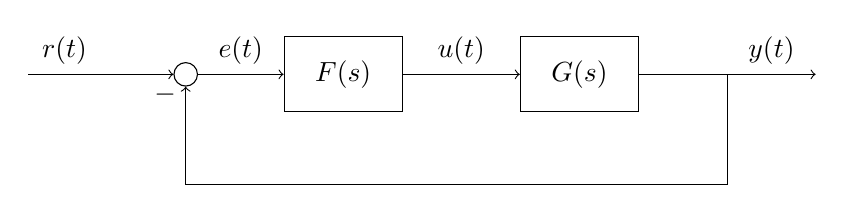
\begin{tikzpicture}[node distance=20mm,
                    block/.style={rectangle, draw, minimum width=15mm, inner sep=3mm},
                    sumnode/.style={circle, draw, inner sep=3pt}]
  \node[coordinate] (input) {};
  \node[sumnode, right of=input] (sum) {};
   \node[block, right of=sum,] (lti) {$F(s)$};
   \node[block, right of=lti, node distance=30mm] (lti2) {$G(s)$};
   \node[coordinate, right of=lti2, node distance=30mm] (output) {};
   \draw[->] (input) -- node[near start, above] {$r(t)$}  (sum);
   \draw[->] (sum) -- node[ above] {$e(t)$}  (lti);
   \draw[->] (lti) -- node[ above] {$u(t)$}  (lti2);
   \draw[->] (lti2) -- node[coordinate] (meas) {} node[near end, above] {$y(t)$} (output);
   \draw[->] (meas) -- ++(0, -14mm) -| node[left, pos=0.96] {$-$} (sum);
 \end{tikzpicture}
\end{center}
\end{frame}


\begin{frame}[label={sec:orgb47f665}]{Block-diagram algebra}
\begin{center}
  \includegraphics[width=.6\linewidth]{../../figures/block-simple-feedback}
\end{center}

Transfer function from \(r(t)\) to \(y(t)\):
\[ \frac{Y(s)}{R(s)} = \frac{G(s)}{ 1+ G(s)}\]

\pause
\alert{Mason's} gain formula for simple systems with one loop only: \[G_c(s) = \frac{\text{Forward path gain}}{1+\text{Loop gain}}\]
\end{frame}




\begin{frame}[label={sec:org2834271}]{Block diagram algebra}
\alert{Activity} Pair the block-diagram with the correct closed-loop transfer function!


\begin{longtable}{cccc}
\textcolor{red}{A} & \textcolor{red}{B} & \textcolor{red}{C} & \textcolor{red}{D}\\
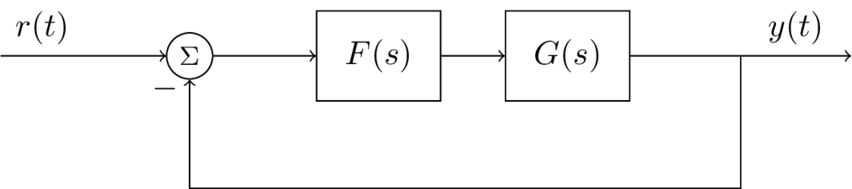
\includegraphics[width=3cm]{../../figures/block-simple-control-feedback} & 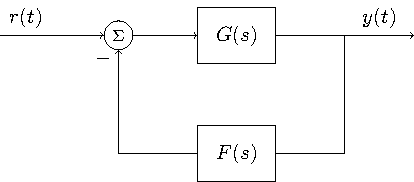
\includegraphics[width=3cm]{../../figures/block-simple-control-feedback2} & 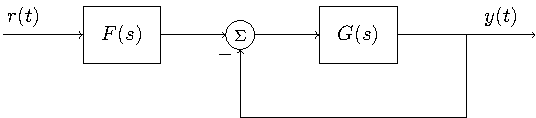
\includegraphics[width=3cm]{../../figures/block-simple-control-feedback3} & 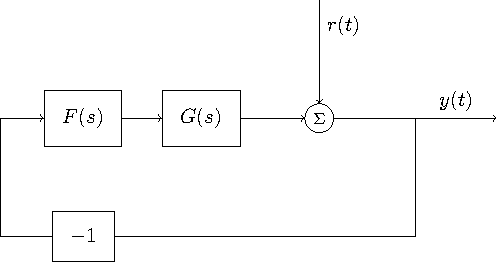
\includegraphics[width=3cm]{../../figures/block-simple-control-feedback4}\\
\end{longtable}


\begin{longtable}{cccc}
\textcolor{blue!80!black}{I} & \textcolor{blue!80!black}{II} & \textcolor{blue!80!black}{III} & \textcolor{blue!80!black}{IV}\\
\(\frac{Y(s)}{R(s)}=\frac{G(s)F(s)}{1 + G(s)}\) & \(\quad \frac{Y(s)}{R(s)}=\frac{G(s)}{1 + G(s)F(s)}\quad\) & \(\frac{Y(s)}{R(s)}=\frac{1}{1 + G(s)F(s)}\) & \(\frac{Y(s)}{R(s)}=\frac{G(s)F(s)}{1 + G(s)F(s)}\)\\
\end{longtable}
\end{frame}
\end{document}